\chapter{Development and Solution}
\label{sec:solution}

After performing research into the problem we now have a better understanding of exactly what needs to be done, and some of the theoretical and implementation based conditions that must be adhered to. It is clear that current implementations of DSM algorithms cannot be put to practical use due to computational intractability with standard sequential hardware, and that a move towards parallelisation has significant potential benefits. But in order to approach the algorithmic problem, first a DSL simulation framework must be created within which to experiment, and this is no small undertaking.

To start with, a stable software base must be selected, that incorporates rapid development due to the expansive scale of this project without sacrificing too much in the way of performance, as well as interoperability with the CUDA API, and is supported by a strong community that can be leveraged to ensure that development is not halted by 'silly' problems.

In \cite{AM09}, McKinley had the same task on his hands, and due to its close-to-the-hardware speed, selected the C programming language. While this was indeed a very fast \footnote{Technically record breaking}, C can often be prohibitively obtuse, with many arcane design patterns and structures that do not aid in rapid prototyping. 

Instead, the Python programming language was selected (in agreement with Dr McKinley) as the base of this project. Python is an interpreted, high-level language, originally created by Guido van Rossum in the 1980's. Two of the biggest draws to Python as a general-purpose language are its flexibility\footnote{Python supports Imperative, Object Oriented, Aspect Oriented and Functional Programming constructs interchangeably} and its extension interface; a significant amount of Python's standard module library is built in C/C++, such that these modules are effectively as fast as straight-C implementations. This is of particular importance with the most popular scientific math library in Python, called Numpy, which is entirely C based and operates very close to the metal, including transparent C-variable assignments and other functionality that preserves the speed of C and the higher level functionality of Python. Additionally, the wealth of Python Profiling\footnote{Profiling is the process of recording a software execution and monitoring the performance and runtime of its constituent functions, providing the developer with a 'look under the hood' to establish what areas of code could be optimised to give the maximum performance improvement with minimum wasted time} tools available means that iterative optimisation (at least of the Python section of the framework) would be painless and fast.

So far, it has been established and justified that Python satisfies the first of the conditions for a stable project base; performance rapid development. To satisfy the second, a Python project called PyCUDA should be noted. 

PyCUDA is a complete CUDA API wrapper for Python, incorporating advantages such as automatic device selection and initialisation, dynamic memory management, kernel templating and direct variable passing, Just In Time (JIT) kernel compilation and invocation, and run-time access to device characteristics and status for dynamic block and grid dimensioning. Unfortunately PyCUDA is lacking in some areas, particularly debugging support, Python Profiling integration (i.e CUDA code will have to be profiled and analyses separately from any other functionality), and automatic multiple device allocation.

Considering these together, the Pros of Python + PyCUDA greatly outweigh their disadvantages. That said, the largest disadvantage is the lack of truly automatic multi-device provisioning, and this is not a major obstacle. Consider this scenario; A single CUDA kernel execution outside of PyCUDA\nomenclature{PyCUDA}{CUDA wrapper for the Python programming language} could execute on multiple devices \footnote{This is technically true only for the latest version of CUDA; at time of writing, 4.0 RC2}, for the planned problem complexities and  data structures, host-to-device memory transactions would eat up any added performance incurred from this style of execution. It is much simpler (and most likely faster) to partition the problem space across the number of available devices, and with the flexibility of Python, this is workable with only a few lines of additional code.

Outside of the programming language itself, utilising a free and open source Distributed Revision Control (DRC) called Mercurial allows for tracking changes and activity in the project, as well as serving as an automatic backup system, through a service called BitBucket, which also provides and issue tracker and on-site wiki for development related notes and tasks.

\section{Solution Development Task list}
In order to fully specify the development of a solution, a task list with appropriate milestones was required to monitor progress and maintain framework stability. This was implemented specifically so that experimental development (or branching) could be explored freely in different development areas (to be detailed), while still allocating time for framework and algorithm re-factoring to leverage shared-object functional decomposition. This task-list mirrors the expanded project objectives in Section \ref{sec:overview}, with additional developmental details.

\begin{enumerate*}
  \item Framework Development and Verification of CPU-bound algorithms
  \begin{enumerate*}
    \item Implementation of Object Oriented DSL bundle simulation framework, with software hooks for algorithm interfacing and standardised result and instrumentation storage formatting.
    \item \emph{Verify Channel Matrix generation against known dataset}
    \item Pure-Python implementation of OSB
    \item \emph{Verify OSB bit-loading against known dataset}
    \item Pure-Python implementations of MIPB and ISB
    \item \emph{Verify results against known dataset}
    \item Refactor algorithm object structure to reduce functional duplication
  \end{enumerate*}
  \item Development and Verification of GPU-bound algorithms
  \begin{enumerate*}
    \item Single GPU implementation of OSB
    \item \emph{Verify results against CPU version}
    \item Multi-device development and implementation of OSB
    \item \emph{Verify results against CPU version}
    \item Single GPU implementation of ISB
    \item \emph{Verify results against CPU version}
    \item Refactor algorithm object structure to reduce functional duplication
  \end{enumerate*}
\end{enumerate*}


\section{Simulation Framework Architecture}
\label{sec:arch}
The architecture of the solution will consist of a simulation framework, emulating the gain-characteristics of an arbitrary DSL bundle structure, with software hooks exposed to any algorithms implemented. 

The fundamental datum required for DSM algorithms is a matrix of crosstalk gains between all lines. This matrix must be generated incorporating the physical relationship of different lines to each other, as well as simulating the material characteristics of the lines themselves in order to calculate the direct gains (i.e the 'cross talk gain' between line \(n\) and itself, or the matrix diagonal).

Once generated, this matrix would describe the bundle of lines, and this inherent value led to the decision to develop the Simulation Framework as an Object Oriented model; the bundle object contains line objects that have individual values, such as their line and network termination locations, noise characteristics, computed SNR, preferential line rates, etc... Additional to these values, each line object exposes internal functions that perform operations on 'itself', such as calculating the far end crosstalk experienced by that line on a particular channel, and the RLCG transfer function over its length. 

The bundle object itself defines the system configuration, and is created from a list of line values read from a file; initially it is planned that this file would contain the LN/NT distances of the line, and if required, the desired rate for that line, but the same theory could be applied to allow mixed material bundles, per line noise characteristics, and other pertinent values. The bundle object's main aims are to initially generate the cross-talk matrix, and subsequently act as an abstraction layer between the DSM algorithm and the individual line values; i.e. the bundle keeps internal arrays to store the power and bit ratings for each line for each channel, which can be operated upon by an external algorithm, and subsequently updated by the bundle itself.

The initialisation of the bundle object (i.e. the generation of the cross-talk gain matrix) can be thought of as a triply nested loop of transfer function calculations, and can be summed up in one sentence: On each sub-channel, for each line (the victim) calculate all the inter-line transfer functions between the victim and every line in the bundle (including itself, but that’s slightly different).

Calculating the direct gain (i.e. the transfer function between the line and itself), the line object simply returns its own transfer function across its length. However, for inter-line (FEXT only, in this project) transfer function calculation, the situation is more complex since lines don't necessarily have the same run length and location; there are nine possible combinations of over-lay between two given lines (plus the case where they don't share any length, hence no FEXT). These are detailed in \cite{RB03} and indicated in Figure ~\ref{fig:FEXT-xtalk-gain}, and this structure was the basis for McKinley's work in this area, but an improved, 'case-less' implementation was generated to segment the line lengths into head length (i.e where one line goes further than the other towards the CO end of the bundle), shared length (where both lines occupy the same sector of the bundle), and tail length( where one line goes further towards the CP end). Each length subsequently has a sector insertion loss (transfer function) and these are multiplied to give the final line transfer function which, incorporating a NICC\footnote{NICC is a UK based communications interoperability standards body} FEXT model function, provides the full length gain response between the two lines on a particular channel.

The operation of segmenting these lengths and producing the cumulative transfer function is numerically subtle but conceptually simple, and with the transfer function configured to return 1 for invalid length values (i.e non-positive lengths), the cumulative transfer function product is effectively self selecting which (if any) sector length values to 'ignore' given different theoretical cases. 

Mathematically,the generation of the inter-line transfer function proceeds thus; 

\begin{equation}
  \begin{array}{l}
  L_h=(V_{lt}-X_{lt})\\
  L_s=\text{abs}(\max(V_{lt},X_{lt})-\min(V_{nt},X_{nt}))\\
  L_t=(V_{nt}-X_{nt})\\
  \end{array}
\end{equation}\label{eq:sectorisation}
\begin{equation}
  \text{insertion loss}(L,F)=\left\{
    \begin{array}{l l}
      \text{transfer function}(L,F) & \quad \text{if}\ L>0\\
      1 & \quad \text{if} L\le 0\\
    \end{array} \right.
\end{equation}\label{eq:insertionloss}
\begin{equation}
  \begin{array}{l}
  H_h=\text{insertion loss}(L_h,f_k)\\
  H_s=\text{insertion loss}(L_s,f_k)\\
  H_t=\text{insertion loss}(L_t,f_k)\\
  H_{\text{total}}=(H_h \times H_s \times H_t)\\
  \end{array}\label{eq:transferproduct}
\end{equation}


This is explained diagrammatically in Figure \ref{fig:FEXT-xtalk-gain}, and the source code for this function as used is in Appendix ~\ref{apx:fext-xtalk-gain}.

\begin{figure}[H]
 \centering
 \subfloat[Case 1]{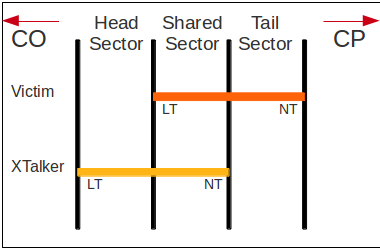
\includegraphics[width=0.35\textwidth,keepaspectratio=true]{images/FEXT_case_1.png}}
 \subfloat[Case 9]{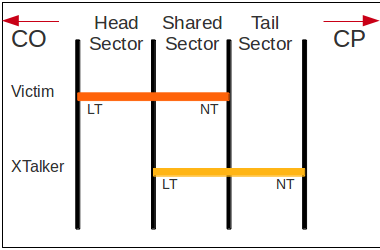
\includegraphics[width=0.35\textwidth,keepaspectratio=true]{images/FEXT_case_9.png}}\\
 \subfloat[Case 2]{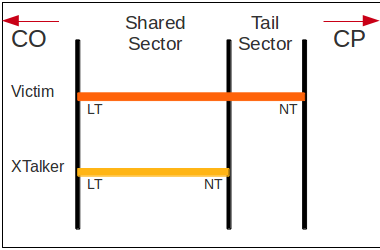
\includegraphics[width=0.35\textwidth,keepaspectratio=true]{images/FEXT_case_2.png}}
 \subfloat[Case 6]{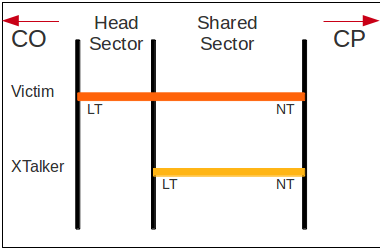
\includegraphics[width=0.35\textwidth,keepaspectratio=true]{images/FEXT_case_6.png}}\\
 \subfloat[Case 3]{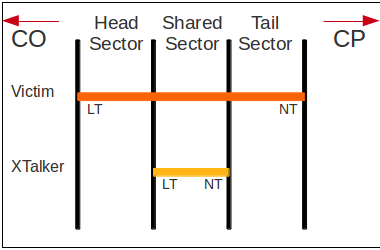
\includegraphics[width=0.35\textwidth,keepaspectratio=true]{images/FEXT_case_3.png}}
 \subfloat[Case 7]{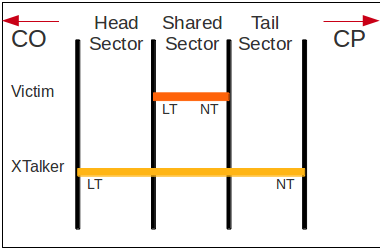
\includegraphics[width=0.35\textwidth,keepaspectratio=true]{images/FEXT_case_7.png}}\\
 \subfloat[Case 4]{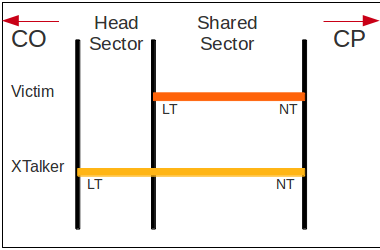
\includegraphics[width=0.35\textwidth,keepaspectratio=true]{images/FEXT_case_4.png}}
 \subfloat[Case 8]{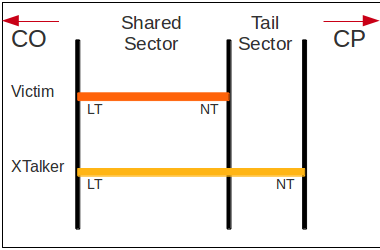
\includegraphics[width=0.35\textwidth,keepaspectratio=true]{images/FEXT_case_8.png}}\\
 \subfloat[Case 5]{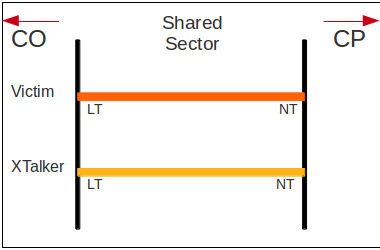
\includegraphics[width=0.35\textwidth,keepaspectratio=true]{images/FEXT_case_5.png}}
 \subfloat[Case 10]{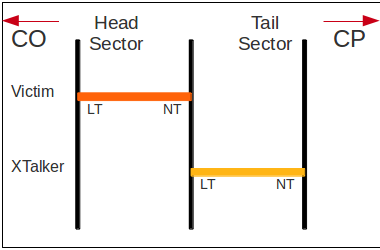
\includegraphics[width=0.35\textwidth,keepaspectratio=true]{images/FEXT_case_10.png}}\\
 % beacons-dist-lin.eps: 0x0 pixel, 300dpi, 0.00x0.00 cm, bb=
 \caption{Case-based explanation of improved FEXT modelling algorithm. Note, Case numbering rearranged to highlight upstream/downstream FEXT case inversion}
\label{fig:FEXT-xtalk-gain}
\end{figure}

As noted previously, incorporation of a Beta probability distribution sample data offsetting can be used to more accurately model the stochastic relationship in inter-line gains based on the locations of those lines in the bundle. This is accomplished by scalar multiplication of the per-channel cross-talk gain matrix with a \(N\times N\) sub-matrix of static gains measured from a 'real' bundle (See Equation ~\ref{eq:ATTFEXT}). One advantageous side effect of this appears in bit-loading of bundles with some 'identical' lines; due to the numerical instability of some bit-loading algorithms and specifically the generation of line power spectral densities, assigned bit-loads can  fluctuate violently between identical lines, producing very impulsive spectra. The relatively tiny gain adjustments applied to different identical lines in the simulated bundle present enough of a 'difference' to overcome this behaviour.

Following from the general Object Oriented architecture, and the bundle object effectively being the fundamental core of the simulation system, this object also maintains control of GPU-based algorithm specific functions, and in the case of multiple GPU operation, maintains persistent thread-pool and task queuing references within a GPU object.

The Initial stage of verification for the system was the comparison of generated Channel Matrices to those found in \cite{AM09}. Due to the different math libraries utilised between McKinley's implementation and this, direct comparison on numerical results is not reliable as a verification method, but test results obtained match those from McKinley to within IEEE floating point specifications. A better comparison is a visual one (Figure ~\ref{fig:cmComparison}).

\begin{figure}[h!]
  \centering
  \subfloat[McKinley]{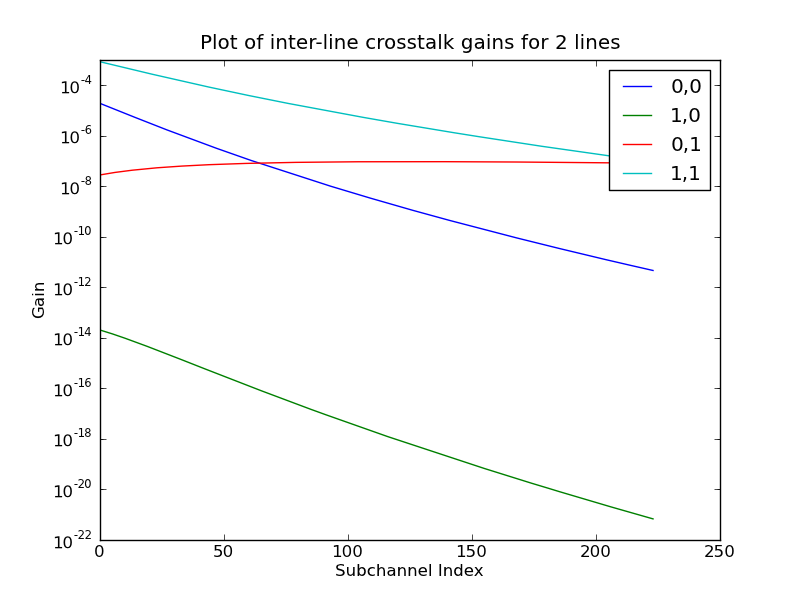
\includegraphics[width=0.45\textwidth, keepaspectratio=true]{images/2_line_channel_matrix_AMK.png}}
  \subfloat[Implementation Results]{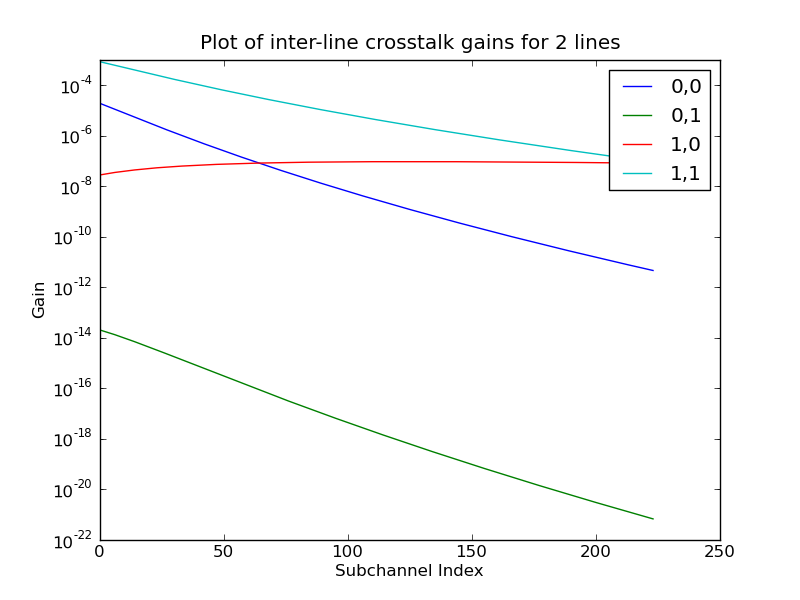
\includegraphics[width=0.45\textwidth,keepaspectratio=true]{images/2_line_channel_matrix_MINE.png}}
  \caption{Visual comparison of known-good channel matrix (McKinley) and Python implementation show that they are identical}
  \label{fig:cmComparison}
\end{figure}


\section{CPU-bound Algorithm Development and Verification}
\label{sec:algo-dev-cpu}
Before tackling the GPU implementation head on, in order to gain a more in-depth and practical understanding of the different DSM algorithms, pure Python, CPU-bound implementations of OSB, ISB and Greedy bit-loading were created. Due to the previously mentioned Object Oriented model, this process was greatly simplified by having each different algorithm class being a 'child' of a generic 'Algorithm' class; inheriting from that parent operations common to all algorithms, such as defining and instantiating universal variables, performing timing operations, verifying PSD 'sanity', file I/O functionality, and general 'build-up/tear-down' operations. This reduced the complexity of each algorithm class (slightly) and ensured that each algorithm was being tested in a consistent and repeatable fashion.

Since OSB is the 'simplest' DSM algorithm, it was implemented first (without per line rate targeting\footnote{Rate Targeting is not a focus of this project, but was explored for fun anyway}, but with PSD caching), largely from the work covered in \cite{AM09}, with operation as stated previously. Due to Python's efficient syntax and the functionality available in the Numpy math library, this was a fairly straightforward task in terms of implementing mathematical formulae in a structured way, but with commonly neglected areas such as algorithmic convergence and numerous boundary cases that are not covered in any of the technical papers cited, this was a process of iterative 'run it; it breaks; find new edge case; implement edge case; repeat'. Such edge cases range from ensuring that while PSD's can have negative values, that a negative PSD value indicates a 'failed' bit-load\footnote{And propagating this information back to the algorithm root before wasting any more processing time on this attempt} to ensuring that assigned line Lagrangian co-factor bisection did not reduce factors to infinitesimal values given very different line sections. 

The in this case, the generation of power spectral density values for each attempted bit combination is accomplished using the Numpy linear algebra library. This development and implementation was carried out in parallel with the generation of the general simulation framework. This joint development allowed for very early-stage verification of the work currently applied, specifically verification of cross-talk matrices and subsequent bit-loads against values derived from \cite{AM09} and \cite{RC04}.

The development of the line and bundle objects, as well as the general framework structure, allowing for programmatic 'hooks' for objects (classes) for different algorithms, automatic generation of post-bit-loading graph data represents more than half of the development time applied to the project\footnote{Seeing it condensed into just over a page of text is slightly depressing!}.

Verification of the OSB algorithm was done in a similar way to the verification of the gain-matrix generation; comparison with known-good results. In this case this takes the form of analysing the resultant PSD and bit assignments for the lines graphically, as shown in Figure ~\ref{fig:osbComparison}. While these do not match each other perfectly, this can be explained by two factors;propagated floating point representation differences, and updated beta-offset implementations. The McKinley implementation was built on a 32-bit floating point representation system, while the presented implementation leverages Numpy's support for 64-bit floating point values. Additionally the selected beta-offset model application in the bundle differs from the McKinley implementation in that in the McKinley model, random beta offset values are applied to the lines sequentially where in this implementation, an offset matrix is applied globally to the bundle using Numpy functionality. Given the inherent numerical instability of the calculation of the Lagrangian sum, fractional changes in cross-talk gains can significantly affect the final resultant bit-loading assignments, while maintaining a close rate-approximation between the two implementations.

\begin{figure}[h!]
  \centering
  \subfloat[McKinley Bit-loading]{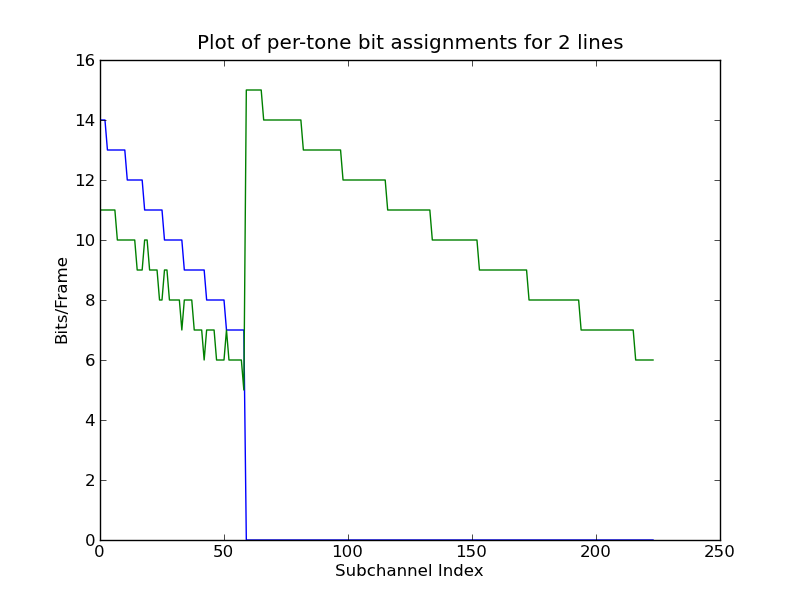
\includegraphics[width=0.45\textwidth, keepaspectratio=true]{images/2_line_bitload_AMK.png}}
  \subfloat[Implementation Bit-loading]{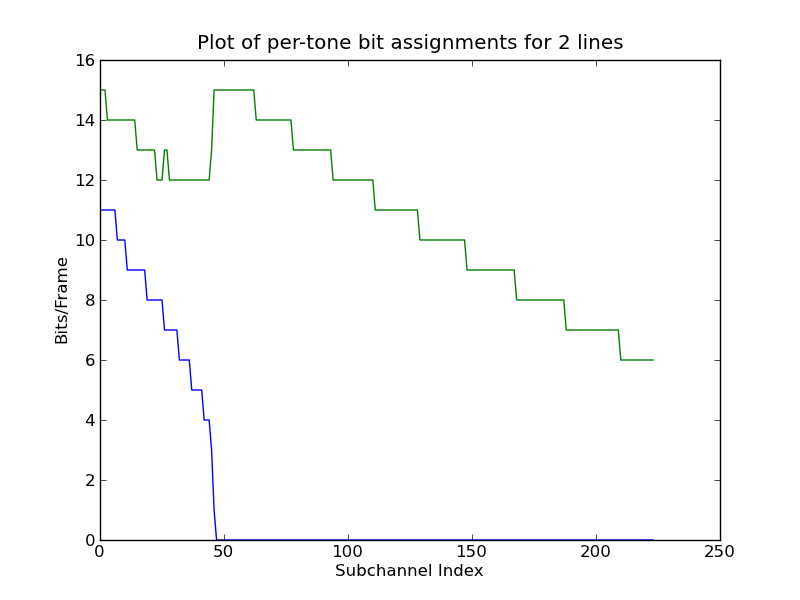
\includegraphics[width=0.45\textwidth,keepaspectratio=true]{images/2_line_bitload_MINE.png}}\\
  \subfloat[McKinley PSD]{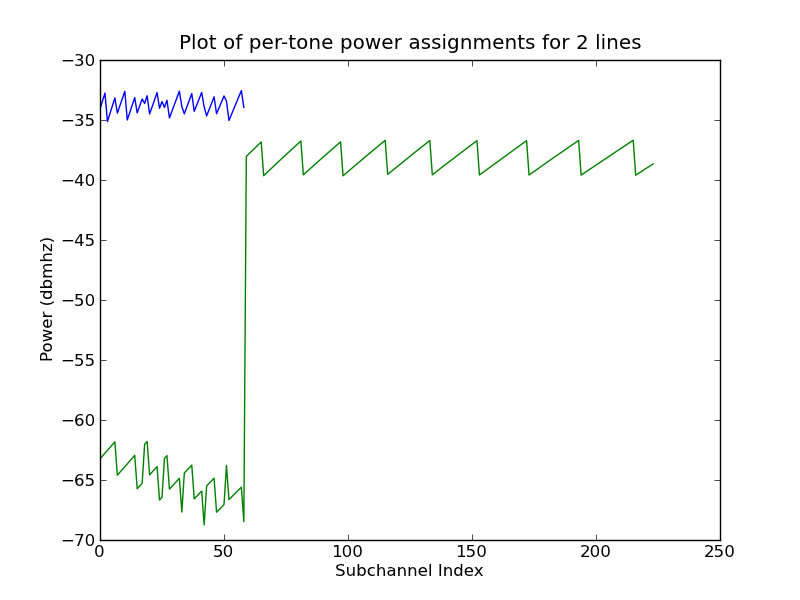
\includegraphics[width=0.45\textwidth, keepaspectratio=true]{images/2_line_power_AMK.png}}
  \subfloat[Implementation PSD]{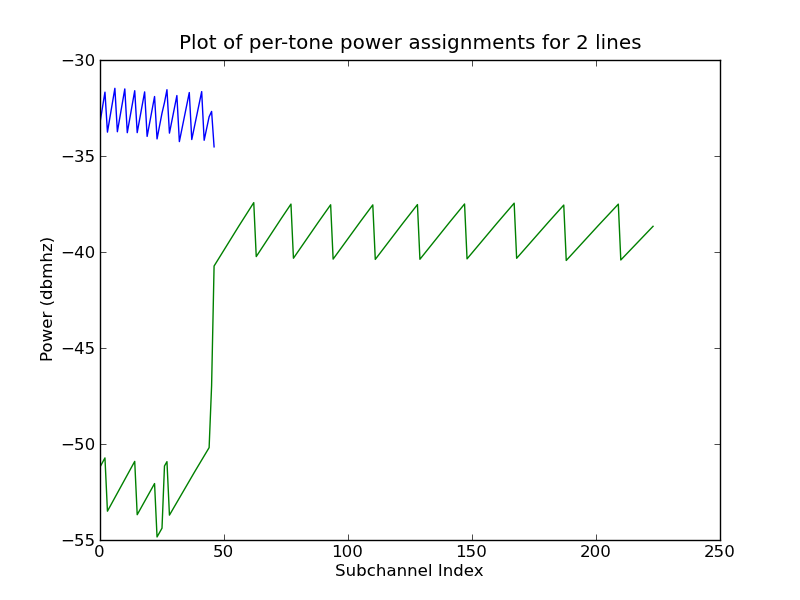
\includegraphics[width=0.45\textwidth,keepaspectratio=true]{images/2_line_power_MINE.png}}\\
  \caption{Visual comparison of known-good (McKinley) and Python implementations of OSB show that they are near-identical}
  \label{fig:osbComparison}
\end{figure}

After OSB was implemented, verified and their operation confirmed by Dr McKinley, Greedy bit-loading (MIPB) with rate targets was developed from \cite{AM09}. One modification that was made to MIPB as in \cite{AM09} was the introduction of a modified line weight updating algorithm that used the ratio-to-target rather than distance-to-target as a weight-shifting factor, giving on average half the number of iterations while maintaining expected bit-loads.\footnote{It is for this reason that MIPB results tend to be slightly skewed with respect to the McKinley implementation.}

\begin{comment}
In \cite{AM09}, three weight update schemes were presented, see Figures ~\ref{fig:mipb-rate-1}, ~\ref{fig:mipb-rate-2}, but during developement of this application, it was found that these update schemes do not converge as quickly as they could, and an alternative rate update scheme, shown in Figure ~\ref{fig:mipb-rate-mine} was implemented that, in a standard four line, three kilometer/five kilometer near-far arrangement, as in ~\ref{fig:4-3k5k-nearfar} with weights selected to be close to optimal, this alternative update converges in FIXME \% fewer iterations than the previously stated versions. As this is not a focus of this project and was simply an investigative whimsy, this will not be investigated further, other than to say that returned results are close enough to previous versions to be considered equivalent.

  \begin{figure}[h!]\label{fig:mipb-rate-1}
    \begin{algorithmic}
      \STATE FIXME
    \end{algorithmic}
  \end{figure}
  \begin{figure}[h!]\label{fig:mipb-rate-2}
    \begin{algorithmic}
      \STATE FIXME
    \end{algorithmic}
  \end{figure}
  \begin{figure}[h!]\label{fig:mipb-rate-mine}
    \begin{algorithmic}
      \FOR {\(n=1\dots N\)}
        \IF{Line Target Set}
          \STATE{\(\Delta b_n=b_n-\text{target}_n\)}
          \STATE{\(\alpha_n=\frac{\delta b_n}{\text{target}_n}\)}
          \IF{\(\text{abs}(\Delta b_n) > b_{\text{tol}}\)}
            \IF{\(\alpha_n ==  1\)}
              \STATE{\(w^+_n=1\)}
            \ELSIF{\(\alpha_n > 0\)}
              \STATE{\(w^+_n=w_n*\alpha_n\)}
            \ELSE
              \STATE{\(w^+_n=w_n*(1-\alpha_n)\)}
            \ENDIF
          \ELSE
            \STATE{\(w^+_n=w_n\)}
          \ENDIF
        \ELSE
          \STATE{\(w^+_n=w_n\)}
        \ENDIF
      \ENDFOR
    \end{algorithmic}
  \end{figure}
\end{comment}

An implementation of ISB soon followed, and verified in the same manner. One particular additional version was made of the ISB algorithm in preparation for GPU parallelisation; loop reversal of the inner optimisation step. 'Classic' ISB iterates over each line individually, internally repeating bit incrementing steps until bit-load convergence is achieved, shown in Figure \ref{fig:isb-standard-loop}. An alternative but equivalent loop construct is to do the per-channel incrementing inside a global bit-convergence loop, as shown in Figure \ref{fig:isb-alternate-loop}. This manipulation is safe since each channel is ideally independent to the power conditions of other tones.

\begin{figure}[ht!]
  \begin{algorithmic}
    \FORALL{channels}
      \REPEAT
        \FORALL{lines}
        \STATE{\(\text{argmax}_{b_k}L(k)\)}
        \STATE{By 1-d exhaustive search}
        \ENDFOR
      \UNTIL{Bit-load Convergence}
    \ENDFOR
  \end{algorithmic}
  \caption{Standard ISB Loop construct}
  \label{fig:isb-standard-loop}
\end{figure}

\begin{figure}[ht!]
  \begin{algorithmic}
    \REPEAT
      \FORALL{channels}
        \FORALL{lines}
        \STATE{\(\text{argmax}_{b_k}L(k)\)}
        \STATE{By 1-d exhaustive search}
        \ENDFOR
      \ENDFOR
    \UNTIL{Bit-load Convergence}
  \end{algorithmic}
  \caption{Exchanged ISB Loop construct}
  \label{fig:isb-alternate-loop}  
\end{figure}

As part of second-stage verification and re-factoring, significant functional portions of OSB and ISB were moved into the Algorithm super-class, such as lambda bisection and rate metric functions, since both algorithms do largely the same thing within the outer loops of the implementation. Since the only differences between the two algorithms is their inner optimisation function, these are included in this document as Appendices \ref{apx:osb-optimise-p-cpu} and \ref{apx:isb-optimise-p-cpu}.

For completeness, figure \ref{fig:mipbComparison} and \ref{fig:isbComparison} show like for like comparison of bit load and power spectra between this solution and the McKinley implementation given a standard two line near-far scenario (as shown in \ref{fig:2-3k5k-nearfar})\footnote{Notice that occasionally the low-channel bit-allocations are swapped between the two lines, i.e. line A in McKinley may have the bit-allocation of line B in this implementation below channel 50. Consultations with McKinley state that this behaviour is acceptable.}

\begin{figure}[h!]
  \centering
  \subfloat[McKinley Bit-loading]{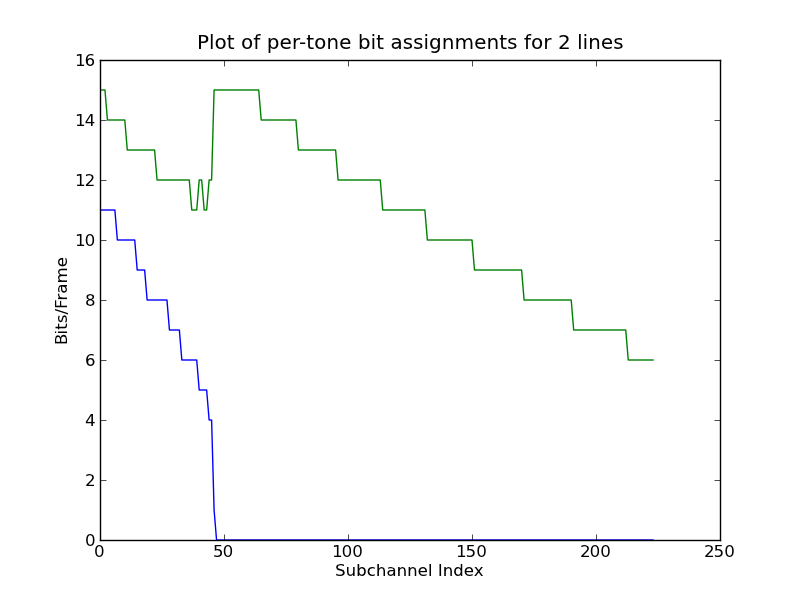
\includegraphics[width=0.45\textwidth, keepaspectratio=true]{images/b_and_p_stats_2lines_near_far_mipb3g_224_371_2451-bitrate.png}}
  \subfloat[Implementation Bit-loading]{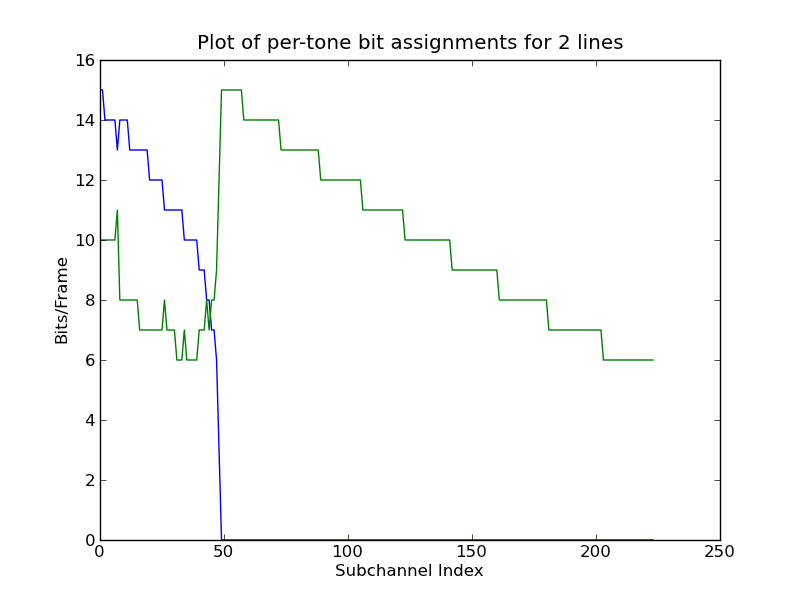
\includegraphics[width=0.45\textwidth,keepaspectratio=true]{images/mipbtest2-bitrate.png}}\\
  \subfloat[McKinley PSD]{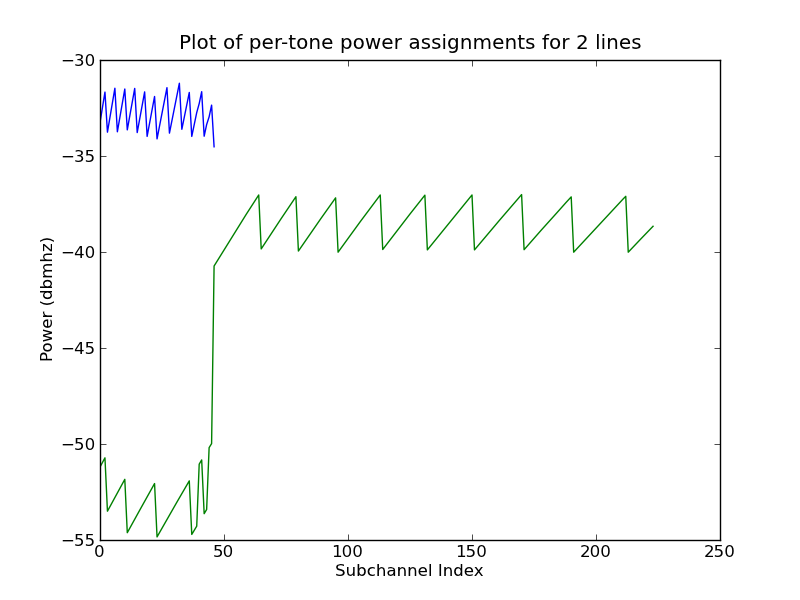
\includegraphics[width=0.45\textwidth, keepaspectratio=true]{images/b_and_p_stats_2lines_near_far_mipb3g_224_371_2451-power.png}}
  \subfloat[Implementation PSD]{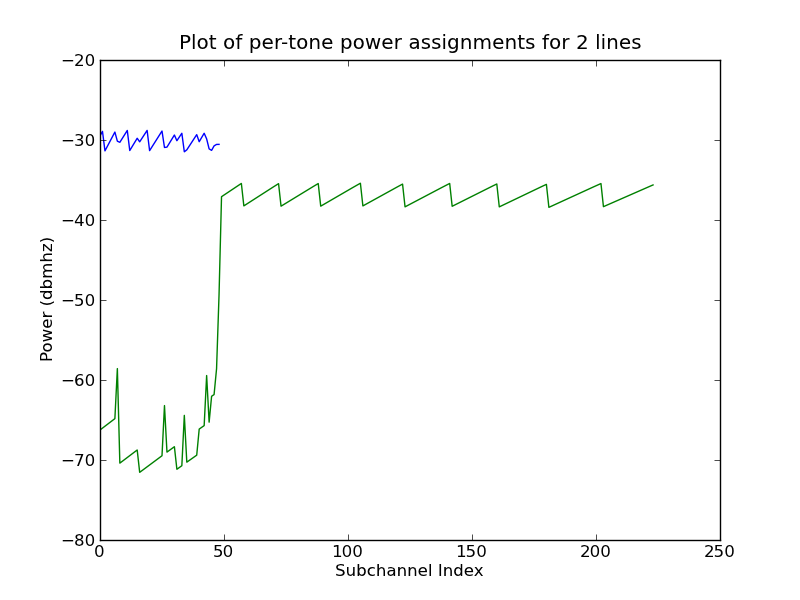
\includegraphics[width=0.45\textwidth,keepaspectratio=true]{images/mipbtest2-power.png}}\\
  \caption{Visual comparison of known-good bit-load and power spectra for Greedy (MIPB), with rates targeted to OSB, show that the implementations are equivalent}
  \label{fig:mipbComparison}
\end{figure}

\begin{figure}[h!]
  \centering
  \subfloat[McKinley Bit-loading]{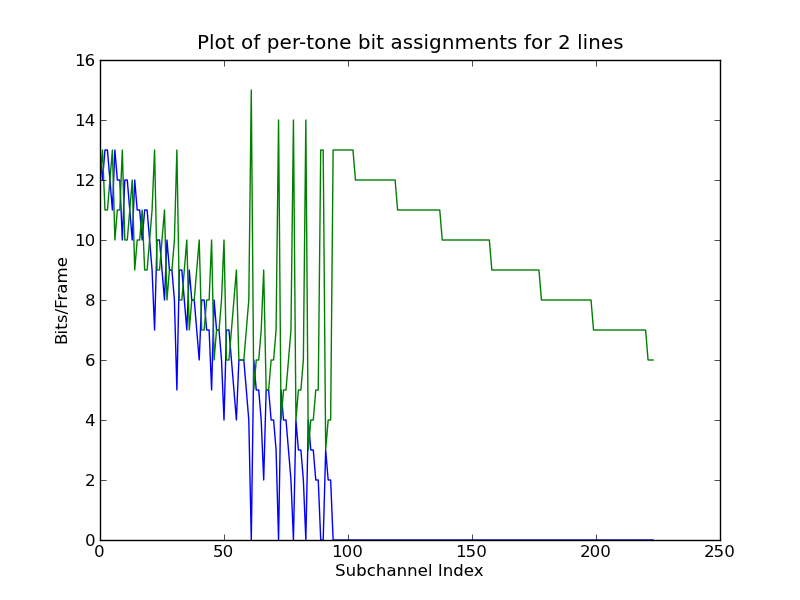
\includegraphics[width=0.45\textwidth, keepaspectratio=true]{images/b_and_p_stats_2lines_near_far_ISB_224-bitrate.png}}
  \subfloat[Implementation Bit-loading]{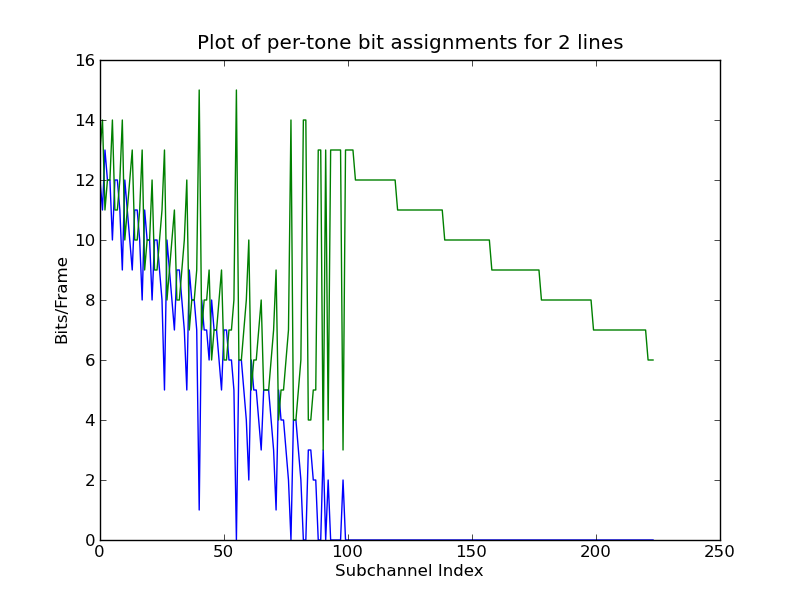
\includegraphics[width=0.45\textwidth,keepaspectratio=true]{images/ISB_2-3k_5k-near_far_CPU-bitrate.png}}\\
  \subfloat[McKinley PSD]{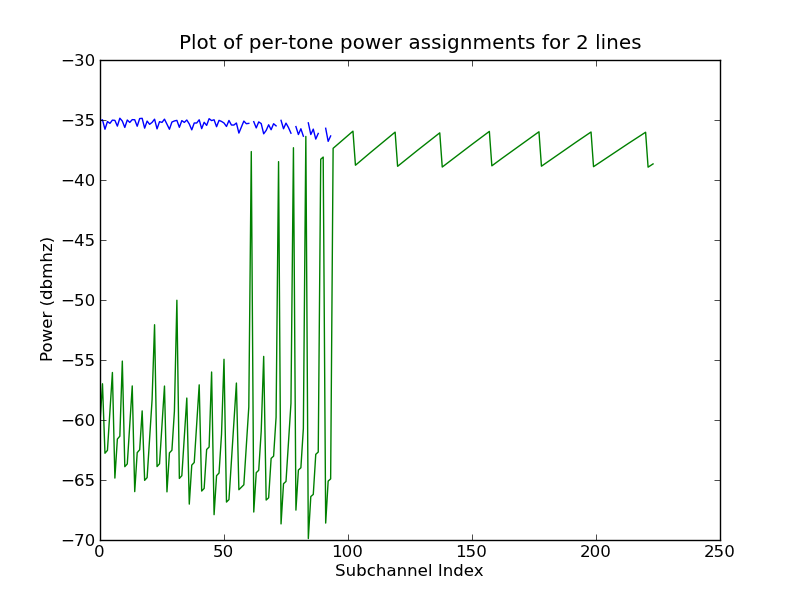
\includegraphics[width=0.45\textwidth, keepaspectratio=true]{images/b_and_p_stats_2lines_near_far_ISB_224-power.png}}
  \subfloat[Implementation PSD]{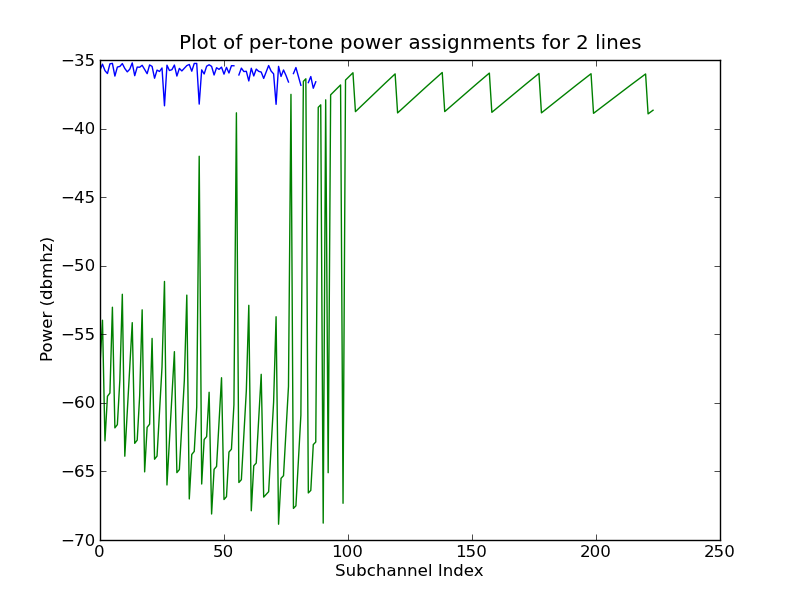
\includegraphics[width=0.45\textwidth,keepaspectratio=true]{images/ISB_2-3k_5k-near_far_CPU-power.png}}\\
  \caption{Visual comparison of known-good bit-load and power spectra for ISB, show that the implementations are equivalent}
  \label{fig:isbComparison}
\end{figure}

\section{GPU-bound Algorithm Development}
\label{sec:algo-dev-gpu}
\subsection{Retrospective analysis of CPU bound applications}
Python's profiling architecture allows for detailed analysis of 'hot-zones' within applications, i.e. the areas within a program where most time and resources are spent over the course of execution. In order to see a 'practical' workload, for the following analysis, a four line near-far bundle was used\ref{fig:4-3k5k-nearfar}.
In order to visualise the profiled-executions, the RunSnakeRun application was used to generate squaremap representations of time spent in different functions; larger areas represent a greater total time spent in that area of computation (Figure \ref{fig:cpuprofileComparison}). 
\begin{figure}[h!]
  \centering
  \subfloat[OSB Profile SquareMap]{\label{fig:cpuprofileOSB}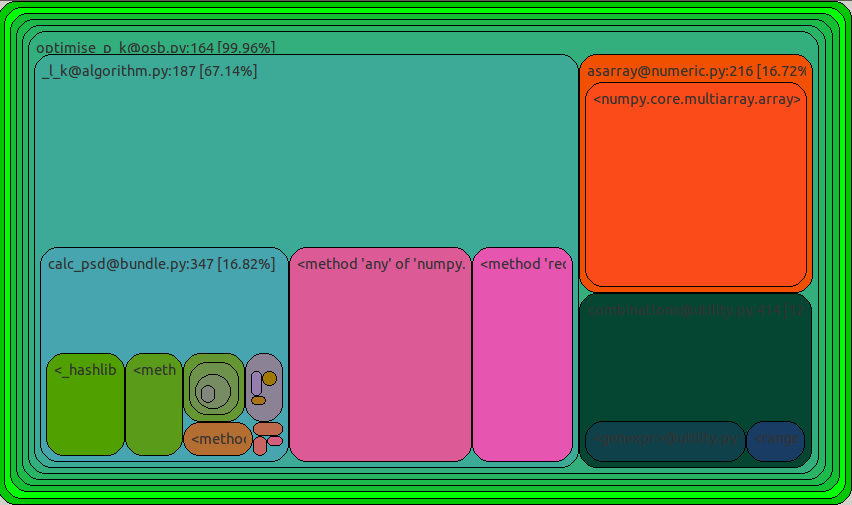
\includegraphics[width=0.75\textwidth,keepaspectratio=true]{images/OSB_4_profile_CPU.png}}\\
  \subfloat[ISB Profile SquareMap]{\label{fig:cpuprofileISB}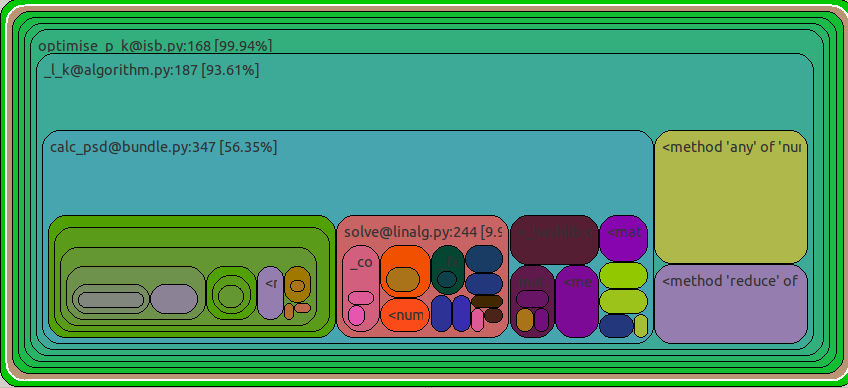
\includegraphics[width=0.75\textwidth, keepaspectratio=true]{images/ISB_4_profile_CPU.png}}\\
  \subfloat[MIPB Profile SquareMap]{\label{fig:cpuprofileMIPB}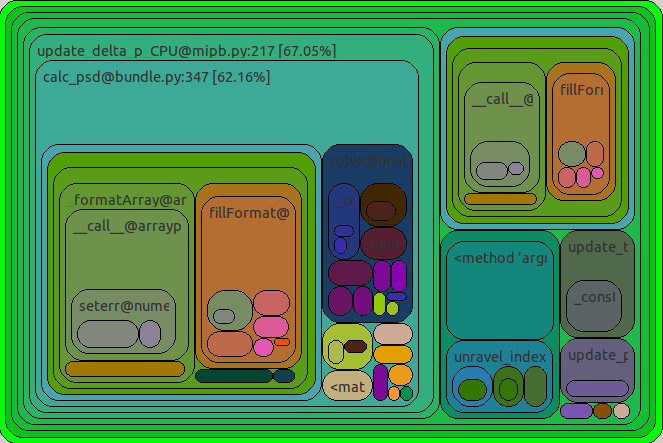
\includegraphics[width=0.75\textwidth,keepaspectratio=true]{images/MIPB_4_profile_CPU.png}}\\
  \caption{SquareMap output from RunSnake showing percentage execution time for a four line bundle scenario}
  \label{fig:cpuprofileComparison}
\end{figure}

\subsubsection{Conclusions}
From these profiling investigations, it is clear that the largest computational bottleneck is the calculation of power spectral densities for different bit-load combinations. This is exemplified particularly in OSB and ISB; the Lagrangian calculations ('L\_k') clearly take up the vast majority of computation time, and in the case of MIPB, the culprit is the recalculation of the \(\Delta p\) values per tone; again, the primary operation is calculation of PSD's. As previously discussed, OSB and ISB, from an algorithmic perspective, lend themselves to parallelisation, but the lack of on-board linear algebra library to calculate individual \(N\times N\)-system solutions is a serious problem; under-test, using the cuBLAS library to calculate \(4\)-system solutions was actually 4\% slower than using the built-in Numpy linear-algebra system on the CPU side\footnote{To try and make this test fair, The calculation was repeated 256 times with pre-generated random inputs on both the GPU and CPU side, with these repeats parallelised on the GPU}. It is clear that for such small matrices, there is no advantage to using standard GPU libraries. And unfortunately, no alternative libraries could be found, and since the CUDA device cannot access any host data, C implementations such as GSL, LAPACK, LINPACK, or EIGEN could not be used.
This leads to the need to create a custom, stripped down, linear system solver\footnote{This was quite possibly the most technically difficult and frustrating section of the entire project}.

Source code is availiable from https://bitbucket.org/bolster/multiuserdsm for all of the applications (and more) used within this project.

Due to the numerical instability of the systems involved, the linear solver must be able to handle arbitrary matrices, as well as being able to gracefully handle failure without bringing the whole GPU down. This led to the selection of a customised maximally pivoted LU Decomposition algorithm\footnote{A Blog post discussing the development of this function is availiable at http://bit.ly/eH3WH6}, pieced together from \cite{WHP92},\cite{GR10}, \cite{JDJZW03} and \cite{GOU96}, and the final solution arrived at is shown in Appendix \ref{apx:cuda-linalg-solver}. This algorithm does not leverage CUDA parallelism. The reason for this is two fold; a natural parallelisation scheme for this algorithm would be for a collection of threads to collaboratively work on a single matrix, but this arrangement would not efficiently occupy the GPU's processing units until the number of lines being tested was greater than at least 8. A Secondary reason is that from the perspective of OSB, having each block calculate a single bit-permutation would greatly limit the number of permutations able to be tested simultaneously, and as such the same kernel that could optimally handle up to \(2^{16}\) permutations (for example, four lines) in one execution would have to be executed eight times to compute the same result. Further, due to the conditional nature of LU Decomposition, utilising per-thread solving on locally related datasets reduces the total amount of warp divergence, increasing overall speed. Experimentally, using block-shared matrix solving was approximately 23\% faster than thread-solving for single executions, but when put into a realistic cradle of input values and ranges, was 15\% slower. This was largely due to the need for repeated executions, as well as the previously stated warp-divergence issues.

The profile results also show that the calculation of optimise\_p is the section of the OSB and ISB algorithms most heavily in need of optimisation. To note in this section is the difference in how the ``asarray.numeric'' numpy functions within optimise\_p are executed between OSB and ISB; these functions are involved in the PSD caching operation; every time a PSD value is requested, the function arguments are hashed, and a dictionary of past values is searched for that hash. This operation greatly reduces the number of linear algebra operations performed in OSB especially (attaining a cache hit ratio of over 98\%, meaning that the algorithm only needs to execute 2\% of the time that it is actually called)\footnote{ISB has a lower, but still significant, cache hit ratio of just over 80\%, but since ISB executes approximately 5\% the number of PSD calculations as OSB, this caching is less significant. MIPB by comparison has a hit ratio of 0\%; no PSD is asked for twice, so caching is largely useless unless using rate targeting, and even then hit ratios average between 10-20\%.}, but does so at the expense of system memory (for a six line network, this cache easily exceeds 8GB). If the calculation of the PSD's can be sufficiently accelerated, this cache could be done away with completely, greatly reducing the total memory footprint of the system, and therefore the cost of execution.

\subsection{OSB: Avenues of parallelisation and problem decomposition schemes}
OSB power optimisation is a naturally parallel algorithm; calculating all possible permutations for all users for all channels, finding the Lagrangian for the best combination on each channel, and loading it. This multiple-level parallelism makes it perfect for GPU execution, but also for multiple GPU execution; each GPU can be assigned blocks of channels or using a channel queue, while each device computes all the permutations for that channel.
Power Optimisation in OSB has three distinct sections; Generation of A and B matrices from individual bit-load permutations, PSD calculation for each permutation, and Lagrangian calculation for that PSD using assigned lambda and weight values. This leads to the possibility of using three independent kernels, with persistent memories across executions (i.e. no need to move memory around during a single optimisation).

This logical decomposition presents another opportunity to leverage the power of CUDA. Using different block and grid dimensions, each kernel's execution could be customised to use a variety of thread and block level parallelism; for instance \(N\) threads could work in parallel within each block to generate the A and B matrices for solving the PSD of each permutation\footnote{As Derived from equation \eqref{eq:DSLSystemModelAlt}}, then individual threads would solve that system, and subsequently calculate the Lagrangian for that permutation, returning a vector of Lagrangian values such that the host process can take the maximum index from that vector and deterministically regenerate the bit-load that created it, as well as retrieving that permutations PSD from the device, completely removing the CPU from PSD generation.

\subsection{Greedy: Avenues of parallelisation and problem decomposition schemes}
Due to the incremental step-wise operation of Greedy bit-loading, and after thorough consultation with Dr McKinley, there is no efficient way to parallelise Greedy without fundamentally changing the operation of the algorithm. To demonstrate this, a 'best-attempt' parallelisation was made, focusing on the updating of tonal costs. After the first step in the algorithm, this is exclusively done on a per-tone basis, meaning that at most, \(N\) values are being generated at once. This produced a slow-down of 23\% when compared to the CPU-bound algorithm against a 6-line bundle, predominantly due to memory transfers between the host and the device.

As such, Greedy must be disregarded from this project, but will be used as a comparison to answer the question 'Can Massive Parallelism compete with algorithmic improvement?'\footnote{Without going any further, I would be confident that this is false for greater than 6 lines; Greedy is just that fast}.

\subsubsection{ISB: Avenues of parallelisation and problem decomposition schemes}
ISB, even though its very close in structure to OSB, presents an interesting predicament; while it is still the power optimisation that is the major workload, the incremental operation of this section of the algorithm makes it initially quite difficult to see how to efficiently parallelise it. At first blush, the same patter as OSB could be followed; where independent channels are separately computed independently, allowing for simple multi-device distribution, or as mentioned, to iterate over the incremental bit combinations of the entire bundle, excluding 'simple' multiple device execution.

In the former case, the style of Figure \ref{fig:isb-standard-loop} would be adopted, where each kernel invocation could iteratively perform optimisation on each particular channel. The difficulty is that this algorithm could not really be parallelised any further due to the incremental nature of ISB. It is possible that this could be split up by each user attempting their own bit-load permutation individually, with a record of 'best' bit-load shared between threads in a block, but this is a fundamental break in the ISB algorithm, so would not be guaranteed to be either near-optimal, or even converge at all.

The second option appears to be the most viable, if (at first glance) less applicable to multiple devices. Using an iteration construct like Figure \ref{fig:isb-alternate-loop}, each thread-block could perform each channel's line-loop optimisation. This would only involve a constantly defined loop within the CUDA kernel, which is significantly more performant than a non-deterministic convergence condition as would be required in the former case. In short, this structure would perform channel and permutation parallelism, with each block containing 16\footnote{The number of possible bit-load combinations for the line currently being looped over within the kernel} threads. While this is not a huge number of threads, it's enough to sufficiently occupy the device. Additionally, CUDA's shared memory space can be used such that at each loop, a block-shared store of the running-bit-load would be updated on each per-line optimisation, containing the bit-permutation with the highest Lagrangian. With 224 ADSL channels, there is no reasonable condition under which this would require more than one device (\(\text{Number of Threads}=B_{\text{max}}\times K\)), but if desired, the channel range could be partitioned across devices.

While the first option will be explored, but the second will be the focus of most development time.

\subsubsection{Development of generalised GPU workload sharing model}
One of the most significant drawbacks of CUDA is its computational simplicity; that is to say that CUDA has relatively little workload partitioning and runtime optimisation when compared to systems such as OpenCL or OpenMP. As such, and from the insights found previously in this section, a generalised workload model was developed to produce near-optimal grid and block dimensions for generic kernels. Although these design patterns are configured with the computation of single PSD/Lagrangian calculations in mind, the same theories of block, warp, grid and device partitioning can easily be applied to any computing problem on GPU's\footnote{as long as those problems are independent of each-other}.

Each CUDA device has an optimal occupancy ratio for a particular kernel, involving the number of SP's available on the device, expected memory accesses, etc., and as such these patterns will not be perfect. They are simply 'quite good', and attempt to dynamically assess optimal block and grid assignments based on individual hardware configurations without having to inspect the kernels being executed. The first of these patterns is a per-device workload calculation. This queries the device for information such as the number of SP's, number of threads per warp, and the maximum permitted threads per block \footnote{Note, this is not the optimal number of threads, just a ceiling value}.

Given a maximum value of 'workload', in this case the number of thread executions ideally desired, the number of warps that this workload requires is calculated. This is scaled to the number of threads per warp and rounded up to the nearest multiple of the warp size (usually 32) to give an optimal 'thread per block' count. This value is then used, along with a maximum thread-count ceiling, termed 'gridmax', to find the optimal number of blocks to execute these threads within while staying within device limits. The python code for this function is shown in figure ~\ref{fig:workload-calc}. Note that this code is developed for 1-D grids and blocks, but could easily be extended for multi-dimensionality or for cooperative thread execution.

\begin{figure}[H]
  \lstinputlisting[language=Python]{sourcefiles/workload-calc.py}
  \caption{Sanitised Python function for near-optimal Grid and Block dimensions for thread-independent operations}
  \label{fig:workload-calc}
\end{figure}

\subsubsection{Development of generalised multi-device function queue}
A GPU device and a host process must be paired, i.e., one host-bound process can execute CUDA kernels on only one GPU device \footnote{This has changed in CUDA 4.0 RC2, but due to PyCUDA's current lack of direct hooks into this functionality, this option could not be explored sufficiently for inclusion in this document}. This restriction, coupled with Python's Global Interpreter Lock (GIL), which is a mutex that prevents multiple native threads from executing Python byte-codes simultaneously\footnote{This is required due to Python's memory management system not being thread-safe}, requires that for multiple GPU devices to me leveraged, additional multi-processing structures must be used.

There are two major families of multiprocessing structures in Python; one that leverages system threads, like Unix pThreads, in a module called 'threading', and a second that uses full processes, akin to OpenMP. The threading model was selected as the use of multiple processes requires that the entire application (or at least the sections of the application that must deal with multiprocessing) be immutable. This disallows the use of class instance methods (such as all of the bundle and algorithm class functions). Further, processes are significantly 'larger' in terms of memory allocation, and significantly slower in terms of process forking, when compared to the lightweight threading model.

As such, the generated GPU class, was augmented with a secondary class of persistent GPU threads. These objects, once instantiated with a GPU device index on application start-up, wait on work items to be put one a queue by the GPU parent class. Once a work item is received, the appropriate internal method for each algorithm is selected and executed on the GPU to which it has been instantiated. The advantage of this queueing method is that work is inherently balanced across devices without any declared load-balancing algorithm since as soon as each thread has completed its current work item and returned its results to the parent class, it simply picks the next free item from the queue.

The overheads incurred in this process are insignificant, and generally hidden; since CUDA executions are none blocking (i.e. unless told explicitly to wait, a host process can continue to process other information during kernel running time), and that these threads are persistent. This persistence is important, since in the single GPU model, each method execution the GPU device must be reinitialised every time the method is called. With this threading model, each device is initialised once during application start-up, and this initialisation time can be hidden behind other work being done such as the generation of the bundle channel matrix.

Further, this threading model allows the application to be device and system agnostic; automatically adapting to a single, twin, or quad-device system with no user action. This combined with the previously mentioned near-optimal workload calculation could even allow for mixed device systems\footnote{Although this functionality has not been tested, since no systems were available for test operated under a mixed-device configuration}.

\section{GPU Solutions and Verification}
The solutions arrived at for GPU consist of a series of C-sourced CUDA kernels, along with a collection of device-side functions. While PyCUDA exposes some high-level GPU abstraction capabilities, such as parallel per-element array manipulations, this avenue of work could not be applied cleanly to the problem set, mainly due to the need for intra-element operations such as PSD solving.

Before diving into details; the OSB solution consists of three separate per-channel kernels that replicate the operation of 'optimise\_p' in the serial implementation (Bit-load/AB generation, PSD Solving, LK calculation), executing for all bit-load permutations simultaneously; while ISB consists of a single kernel that performs per iterative optimisation across a range of channels simultaneously, with the kernel being iteratively executed until bit-load convergence\footnote{Strictly speaking, these calculations are not simultaneous, as individual warps are swapped in and out of the SM's, but for the sake of simplicity, 'simultaneously' is used}.

Additionally, a secondary function was generated for global verification of 'optimal' bit-load PSD's, used during final recalculation of per-line power ratings.

These kernels and device functions are shown in detail in Appendix \ref{apx:GPU-code}

\subsection{OSB GPU}
In the OSB solution, the full permutation range is sliced based on the maximum efficient capacity of the device being used; this generally allows for a maximum three-line solution to be found in 'one shot', but since OSB permutations are computationally explosive, often the kernel triplet is executed many times to span this permutation range to arrive at an optimal solution for a single channel.

This kernel triplet consists of:
\begin{itemize*}
\item{'lk\_osb\_prepare\_permutations': Generate A and B matrices for PSD calculation of all bit permutations}
\item{'osb\_solve': Solve all permutation's PSD's in parallel}
\item{'lk\_max\_permutations': Solve all permutation's PSD's in parallel}
\end{itemize*}
The reason for the separation is partly logically and partly technical; the generation of A and B matrices is made parallel in both the permutation and line ranges, as each A/B generation shares many values for each respective permutation. Therefore the block and grid dimensions for CUDA execution were set so as to enhance memory coalescing and column-major shared memory accesses; each 'block' calculates one permutation, and each thread within the block calculates one row of A and B. The Solving and LK generation kernels do not easily exhibit this level of parallelism and as such are executed under a thread-share model; i.e. each thread is independent but grouped as a 'best attempt' at efficient memory access.

As this algorithm operates on a per-channel basis, the major input data (the cross-talk gain matrix) can stay resident on the device for the complete execution of one channel, reducing the time spent transferring data to and from the device. Additionally, this algorithm allows access to not only the optimised bit-load, but also to the PSD of that bit-load, which remains resident in device memory. This reduces repeat-calculations.

After each kernel execution, as CUDA has no rational way to perform linked-reductions (such as \(\text{argmax}\)), the device array containing LK values is returned to the host, and the maximal LK-permutation found from the array-index. If this LK value exceeds the current global maximal LK, then the PSD for that value is also pulled from the device, and returned to the calling function.

The multi-device extension to this implementation is a simple queue-based channel distribution across devices, as discussed previously. An attempt was made to distribute permutation slices instead of channels, but due to excessive memory redundancies (i.e the same cross-talk gain matrix having to be constantly sent to the host) this implementation was significantly slower that the channel-distributed model\footnote{For four line OSB, the permutation sharing implementation encountered a versus-CPU speed-up of 3x, compared to, as we'll see later, a channel-distributed speed-up of 10 on a single GPU}.

\subsubsection{Verification}
The natural verification method is to compare returned PSD's against the previously-verified CPU implementation (Figure \ref{fig:cpugpuOSBComparison}). What is interesting about this result is that while power allocations match almost perfectly, bit allocations differ, it appears, significantly. This is due to the inherent numerical instability of the Lagrangian maximisation method. In relative terms, single-differences in bit allocations correspond to minimal PSD changes, and the absolute difference in total bit-load between CPU and GPU versions is less than 35 bits-per-frame over the entire bundle.

As this is an investigation into the viability of GPU implementations and not a study in their correctness, it is felt that this is an acceptable margin of error.

This verification stands for both single and multi-GPU executions.
\begin{figure}[H]
  \centering
  \subfloat[OSB CPU Power Allocation]{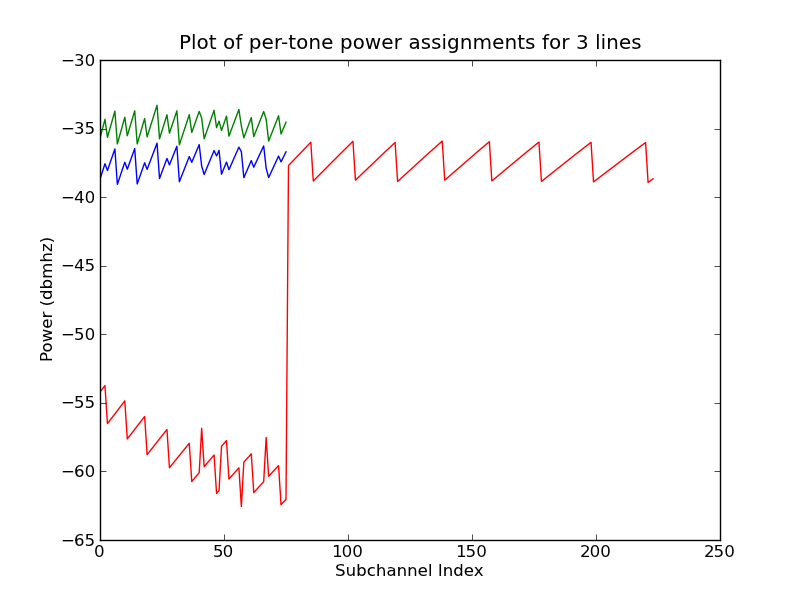
\includegraphics[width=0.45\textwidth,keepaspectratio=true]{images/OSB_3-3k_5k-near_far_CPU-power.png}}
  \subfloat[OSB GPU Power Allocation]{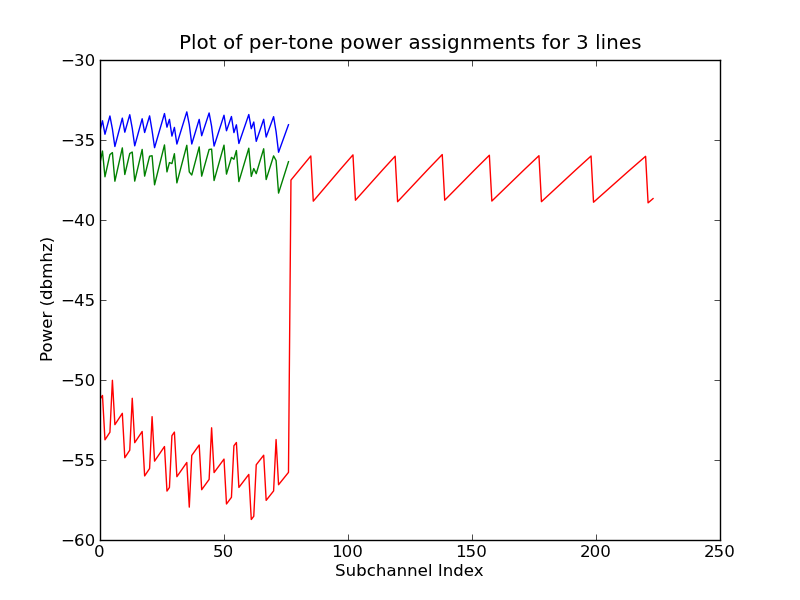
\includegraphics[width=0.45\textwidth, keepaspectratio=true]{images/OSB_3-3k_5k-near_far_GPU-power.png}}\\
  \subfloat[OSB CPU Bit-load]{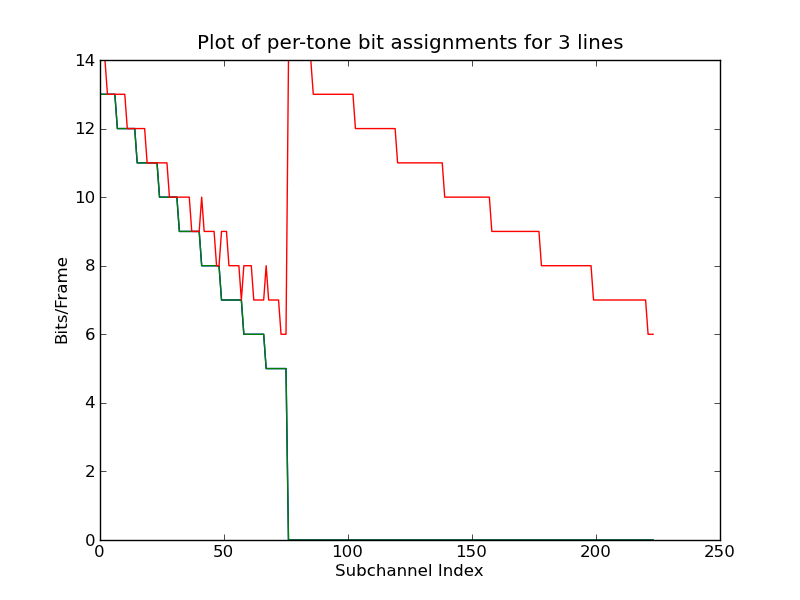
\includegraphics[width=0.45\textwidth,keepaspectratio=true]{images/OSB_3-3k_5k-near_far_CPU-bitrate.png}}
  \subfloat[OSB GPU Bit-load]{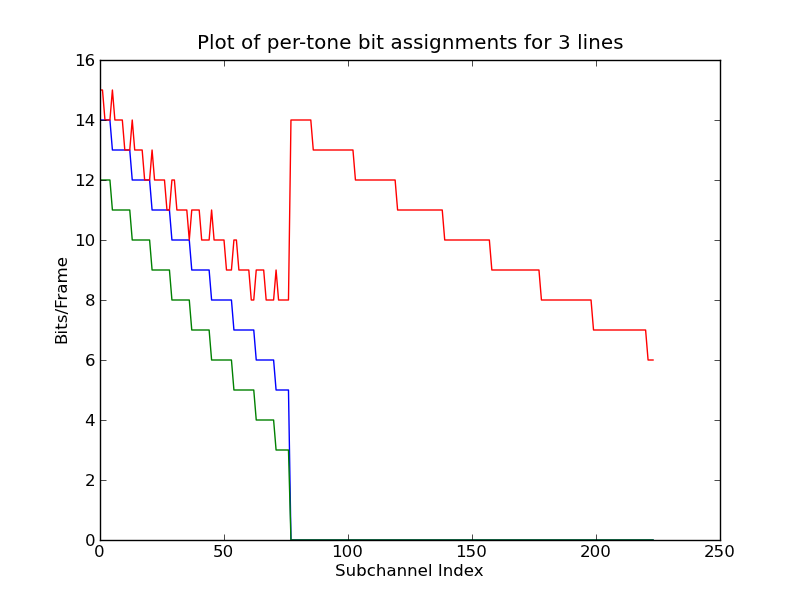
\includegraphics[width=0.45\textwidth, keepaspectratio=true]{images/OSB_3-3k_5k-near_far_GPU-bitrate.png}}\\
  \caption{Comparison of three line, near far scenario OSB: CPU/GPU}
  \label{fig:cpugpuOSBComparison}
\end{figure}
\subsection{ISB GPU}
In the ISB solution, the host thread iteratively calls a single kernel that operates on all channels simultaneously, 'isb\_optimise\_inc', that increments across each line and updates a shared 'optimal' bit-load for that iteration. The kernel is repeatedly called until the bundle/sub-bundle bit-load has converged\footnote{Sub-bundles in the case of multi-GPU operation}.

This kernel operates on a mixed-thread-share model, where each block within the CUDA grid calculates the optimal load for a single channel, and each thread within the block performs the PSD and LK calculations for the line being iterated upon. As such, the 1-D grid takes the form \([K|B_{\text{max}}]\). Each block maintains a shared memory location for the 'best' bit-load permutation from each successive line-round, and thus collects an 'optimal' bit-load across all lines on that channel. As such, strictly speaking this kernel is not limited by the number of lines, but by how long it takes for the bit-loads to converge \footnote{Experimentally it has been found that this implementation of ISB can happily operate on at least 16 line bundles within a practicable time frame(24 seconds), and the only reason for not going further than that is the constraints of 32-bit numerical representation of bit-permutations}

\subsubsection{Verification}
Again, the simplest way to verify operation is direct comparison to CPU bound implementations (Figure \ref{fig:cpugpuISBComparison}) In this case the graphs tell a very different story than that of OSB; as can be seen, the GPU implementation has power convergence problems between the green and red lines, but the bit-loads applied are nearly a perfect match. This is again due to numerical representation problems, where by the PSD/LK calculations produce vanishingly small differences between these two line segments, leading to oscillation of bit-load allocations across these lines. Again, the end result of this is a global bundle rate that is within 3\% margin of error between CPU/GPU implementations.
\begin{figure}[H]
  \centering
  \subfloat[ISB CPU Power Allocation]{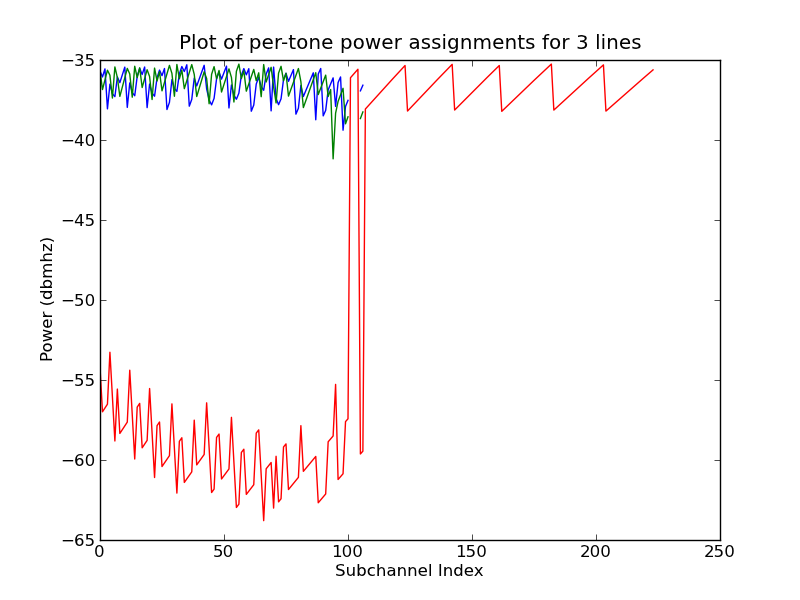
\includegraphics[width=0.45\textwidth,keepaspectratio=true]{images/ISB_3-3k_5k-near_far_CPU-power.png}}
  \subfloat[ISB GPU Power Allocation]{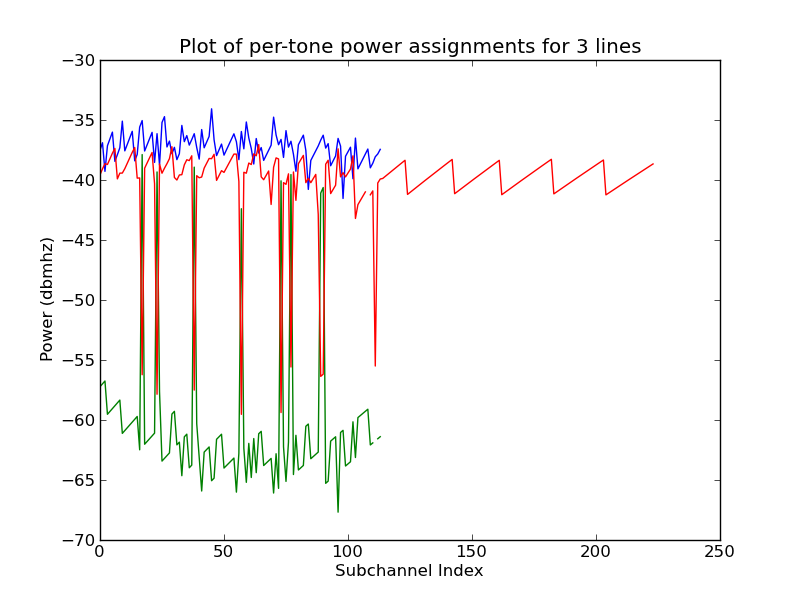
\includegraphics[width=0.45\textwidth, keepaspectratio=true]{images/ISB_3-3k_5k-near_far_GPU_1-power.png}}\\
  \subfloat[ISB CPU Bit-load]{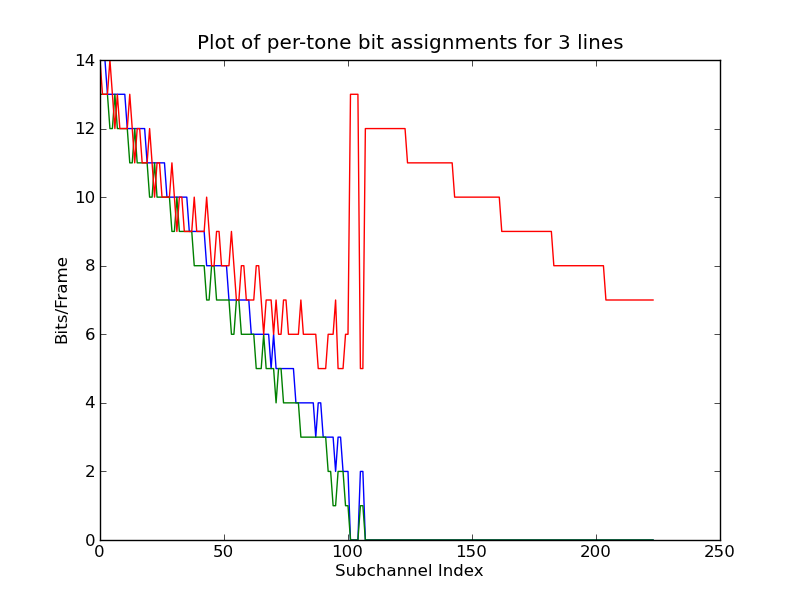
\includegraphics[width=0.45\textwidth,keepaspectratio=true]{images/ISB_3-3k_5k-near_far_CPU-bitrate.png}}
  \subfloat[ISB GPU Bit-load]{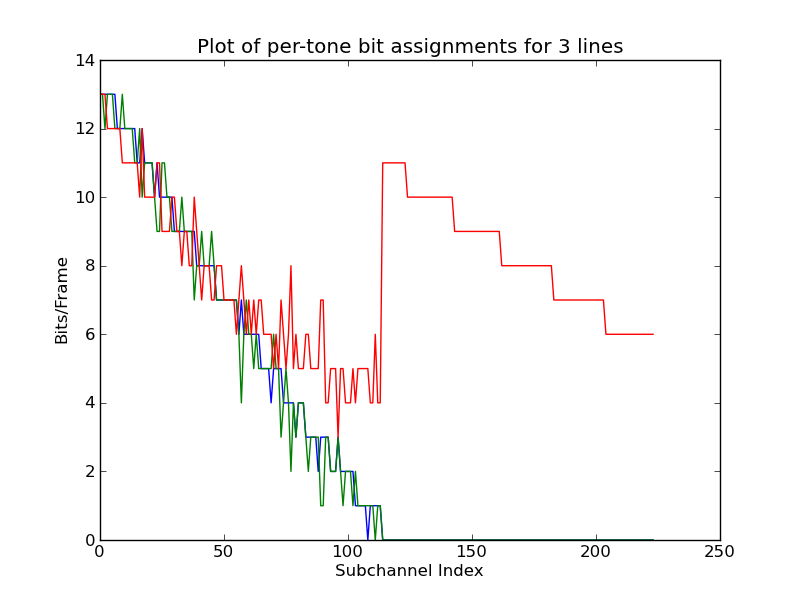
\includegraphics[width=0.45\textwidth, keepaspectratio=true]{images/ISB_3-3k_5k-near_far_GPU_1-bitrate.png}}\\
  \caption{Comparison of three line, near far scenario ISB: CPU/GPU}
  \label{fig:cpugpuISBComparison}
\end{figure}

\subsection{MIPB GPU}
No MIPB solution attempted was functional; as stated, MIPB as it stands has no direct parallelisation vector. Work is under way to perform parallel pre-computation of bit-load chains, but as this is a fundamental divergence from this reports aim, it is not within the scope of this discussion.
